\providecommand{\main}{../}
\documentclass[../writeup.tex]{subfiles}

\begin{document}  


\section{Methods}


\subsection{Joint Demultiplex and Upsample}

One approach which we can consider involves the following steps
\begin{enumerate}
    \item Use $\widetilde{\bC}$ for bucket activities and capture the two-bucket image $\bY$
    \item Recover full resolution images $\bX$ under $S$ illuminations from $\bY$ by solving a linear inverse problem
    \item use $\bX$ to solve for phase and albedo using ZNCC decoding \cite{mirdehghanOptimalStructuredLight2018}
\end{enumerate}
Instead of treating upsampling (recover $2F$ images $\sI$ from $2$ images $\bY$) and demultiplexing (recover $S$ images $\bX$ from $2F$ images $\sI$) as distinct steps, we aim to recover $\bX$ directy from $\bY$, in a single step, by solving a linear inverse problem. Jointly upsample and demultiplex enforces a prior knowledge of image formation and reduces accumulation of error at each image processing step \cite{heideFlexISPFlexibleCamera2014}. This approach allows encoding arbitrary subsampling schemes in the forward operator and can be adapted to any frame number $F$. Assuming an isotropic Gaussian noise model ($\by=\bA\bx + \be$ where $\be\sim \sN(0,\sigma^2 \bI)$), and prior $p_{\rx}(x) \propto \exp\pc{- (\lambda/\sigma^2) R(\bx) }$ where $R:\R^{SP}\to\R$ is some regularizer for $\bx$. Given noisy measurement $\by$, \textit{max a posterior} estimate $\hat{\bx}$ can be obtained by solving the following
\begin{align}
    \hat{\bx}(\by)
        = \argmin_{\bx}
        \frac{1}{2} \norm{\bA\bx-\by}_2^2 + \lambda R(\bx)
    \label{eq:generic_prior_inverse_problem}
\end{align}
where $\lambda$ is weight for the regularizer. We solve (\ref{eq:generic_prior_inverse_problem}) using RED ADMM \cite{romanoLittleEngineThat2016}. We can specialize the update equations to our problem. First we notice that $\bA\bA^T$ is diagonal when $\bW$ is the optimal bucket multiplexing matrix constructed from Hadamard matrix specified in \cite{weiCodedTwoBucketCameras2018}. The x-update can be simplified  \cite{liuRankMinimizationSnapshot2019} 
\begin{align}
    \bx^{k+1} 
        = \tilde{\bx} + \bA^T \begin{bmatrix}
            \frac{(\by - \bA\tilde{x})_1}{\bzeta_1 + \rho},\cdots, \frac{(\by - \bA\tilde{\bx})_{SP}}{\bzeta_{SP} + \rho}
        \end{bmatrix}^T
    \label{eq:red_x_desci_update}
\end{align}
where $\rho$ is the parameter for augmented lagrangian, $\tilde{\bx} = \bz^k - \bu^k$, and $\bzeta = \diag \left(\bA\bA^T\right)$, which can be precomputed. (\ref{eq:red_x_desci_update}) is fast because it consists of 2 sparse matix-vector multiply and a few element-wise vector operations. The update equations is then
\begin{align} 
    \bx^{k+1}
        &= \tilde{\bx} + \bA^T \begin{bmatrix}
            \frac{(\by - \bA\tilde{x})_1}{\bzeta_1 + \rho},\cdots, \frac{(\by - \bA\tilde{\bx})_{SP}}{\bzeta_{SP} + \rho}
        \end{bmatrix}^T
        \qquad \tilde{\bx} = \bz^k - \bu^k \\
    \bz^{k+1}
        &= \frac{1}{\rho + \lambda} \left(
            \lambda \sD(\bz^{k}) + \rho ( \bx^{k+1} + \bu^k  )
        \right) \\
    \bu^{k+1}
        &= \bu^k + \bx^{k+1} - \bz^{k+1}
    \label{eq:red_admm_update_equations_fast_x_update}
\end{align}


\subsection{Experimental Results}

\paragraph{Ground Truth} Ground truth phase/disparity is obtained by computing ZNCC decoding on sinusoids of periods 1,2,5,17,31, each shifted 30 times. Each measurement under a unique illumination pattern is stacked form 250 noisy images. 

\paragraph{Empirical Performance Upper Bound} In Figure~\ref{fig:sinusiods_spatial_freq_1_phase_upper_bound_wrt_S}, we experimentally determine what is empirically possible for the decoding algorithm, without either noise nor recosntruction error, when given measurement under different number of phase shifts, assuming sinusoidal pattern with period 1.

\paragraph{}

\begin{figure}[h!]
    \begin{center}
        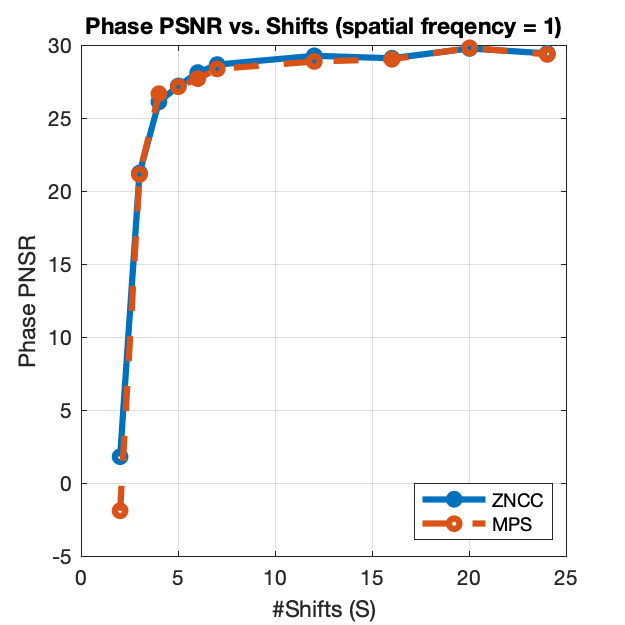
\includegraphics[width=0.49\textwidth]{SinusoidsSpatialFreq1PhaseUpperBoundPSNR}
        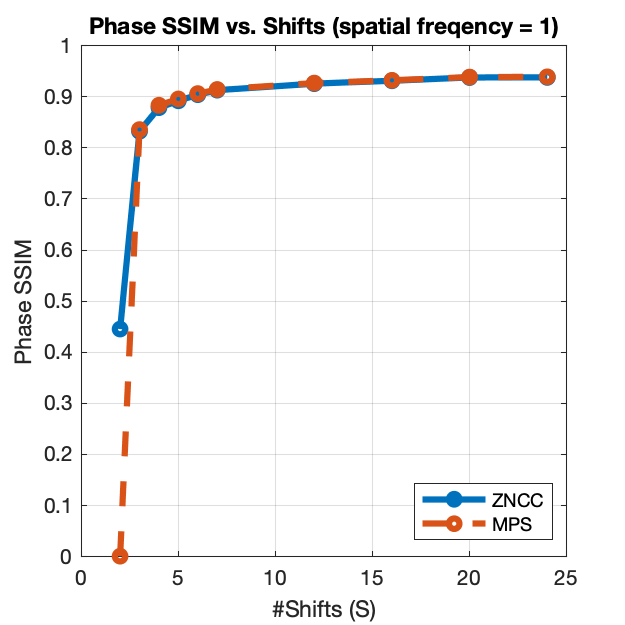
\includegraphics[width=0.49\textwidth]{SinusoidsSpatialFreq1PhaseUpperBoundSSIM}
        \caption{PSNR/SSIM computed by comparing phase obtained by ZNCC/MPS decoding on stacked noiseless images for sinusoidal pattern with period of 1 with varying number of phase shifts to the ground-truth phase. Both decoder performed similarly. We see large improvement when $S=3,4$ and minimal improvement when $S>7$.}
        \label{fig:sinusiods_spatial_freq_1_phase_upper_bound_wrt_S}
    \end{center}
\end{figure}  
 latex

 \begin{table}
    \centering
    \begin{tabular}{c|cccccccccc}
    \hline
     & S=2 & S=3 & S=4 & S=5 & S=6 & S=7 & S=12 & S=16 & S=20 & S=24 \\
    ADMM-MF & 1.92/0.436 & 20.44/0.747 & 24.49/0.828 & 25.47/0.832 & 26.35/0.848 & 26.68/0.848 & 27.19/0.861 & 25.71/0.814 & 24.89/0.802 & 23.67/0.787 \\
    ADMM-TNRD & 1.92/0.436 & 19.13/0.728 & 19.66/0.816 & 20.71/0.812 & 19.35/0.814 & 19.59/0.830 & 21.16/0.856 & 20.00/0.844 & 22.50/0.852 & 23.46/0.845 \\
    \end{tabular}
    \caption{MyTableCaption}
    \label{table:MyTableLabel}
\end{table}

% \subsection{Solving Inverse Problem using RED}

% We first note that the illumination ratios are albedo quasi-invariant, and therefore smooth within object boundaries. Therefore, total variation regularization on illuination ratio images could be particularly effective. To avoid extra notations, we use $\bx,\by$ as the corresponding illumination ratios that we want to reconstruct. Additionally, we adapt algorithm in \cite{romanoLittleEngineThat2016} for imposing algorithm induced priors with state-of-the-art denoisers. In summary, we want to optimize the following constrained problem with a set of affine constraints,
% \begin{align*}
%     \minimize  & \norm{\bA\bx_1 - \by}_2^2 + \frac{\lambda_2}{2} \bx_2^T(\bx_2 - \sD(\bx_2)) + \lambda_3 \norm{\bx_3}_1 \\
%     \subjectto & \bx_1 - \bx_2 = 0 \\
%                & \bG\bx_1 - \bx_3 = 0 \\
% \end{align*}
% where $\bx_1,\bx_2\in\R^{SP}$, $\bx_3\in\R^{2SP}$. $\lambda_2,\lambda_3>0$ are weights to the regularizers. $\bG\in \R^{2SP\times SP}$ is the discrete image gradient for $S$ images 
% \[
%     \bG =
%     \begin{bmatrix}
%         \bI_S \otimes \bG_x \\
%         \bI_S \otimes \bG_y \\
%     \end{bmatrix} 
% \]
% where $\bG_x,\bG_y\in\R^{P\times P}$ are the discrete image gradients for a single image computed using forward difference. We can gather constraints into a single linear system 
% \[
%     \bH\bx = 0
%     \quad\quad \text{where}\quad\quad
%     \bH = 
%     \begin{bmatrix}
%         \bI_{SP} & -\bI_{SP} & 0  \\
%         \bG    & 0    & -\bI_{SP}  \\
%     \end{bmatrix}
%     \quad
%     \bx = 
%     \begin{bmatrix}
%         \bx_1 \\ \bx_2 \\ \bx_3
%     \end{bmatrix}
% \]
% and arrive at an equivalent optimization problem
% \begin{equation}
%     \label{eq:method_optimization_problem}
%     \begin{aligned}
%         \minimize  & f_1(\bx_1) + \lambda_2 f_2(\bx_2) + \lambda_3 f_3(\bx_3) \\
%         \subjectto & (\bx_1,\bx_2,\bx_3) \in \sC
%     \end{aligned}
% \end{equation}
% where $\sC = \{\bx\in\R^{4SP} \;\mid\; \bH\bx = 0\}$ and 
% \begin{align*}
%     f_1(\bx_1)
%         &=\norm{\bA\bx_1 - \by}_2^2 \\
%     f_2(\bx_2)
%         &=\frac{1}{2} \bx_2^T(\bx_2 - \sD(\bx_2)) \\
%     f_3(\bx_3)
%         &=\norm{\bx_3}_1
% \end{align*}

% \subsection{Optimization}

% As shown below, the scaled form ADMM for solving (\ref{eq:method_optimization_problem}) is given by 
% \begin{align*}
%     \bx_1^{k+1}
%         &= \prox_{(1/\rho)f_1}(\bz_1^k - \bu_1^k) 
%         = (I + \frac{2}{\rho} A^TA)^{-1} ( \bz_1^k - \bu_1^k + \frac{2}{\rho}A^T y) \\
%     \bx_2^{k+1}
%         &= \prox_{(\lambda_2/\rho)f_2}(\bz_2^k - \bu_2^k) 
%         = \frac{1}{\lambda_2+\rho} (\lambda_2 \sD(\bx_2^k) + \rho(\bz_2^k - \bu_2^k)) \\
%     \bx_3^{k+1}
%         &= \prox_{(\lambda_3/\rho)f_3} (\bz_3^k - \bu_3^k) 
%         = \sS_{\lambda_3/\rho}(\bz_3^k - \bu_3^k) \\
%     \bz^{k+1}
%         &= \prox_{(1/\rho)\sI_{\sC}}(\bx^{k+1} + \bu^k)
%         = (I - \bH^{\dagger}\bH)(\bx^{k+1}+\bu^k) \\
%     \bu^{k+1}
%         &= \bu^{k} + \bx^{k+1} - \bz^{k+1}
% \end{align*}



\end{document}

